\section{Highlights}
\vspace{-.2cm}
\subsection{``Real'' EARS}
EARS was not originally built to describe requirements at a level where they can
automatically be transposed into a real system. As such, an effort had to be
made in order to overcome the semantic gap between, on the one hand, the
structured but non-formal nature of EARS and, on the other hand, the strictly
formal nature of the Linear Temporal Logic (LTL) formalism needed by the
automated synthesis mechanisms.\vspace{-.5cm}
\begin{figure}[h!]
   \begin{center}
     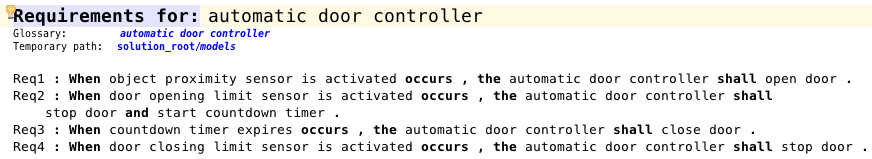
\includegraphics[width=1\textwidth]{images/EARS-Reqs.png}
     \caption{\textsf{EARS-CTRL} Requirements for a sliding door
     controller}
     \label{fig:ears_reqs}
   \end{center} 
 \end{figure}
\vspace{-1cm}Figure~\ref{fig:ears_reqs} illustrates a set of \textsf{EARS-CTRL}
requirements for the software controller for a sliding door. By remaining as close as
possible to the original EARS syntax our editor allows building requirements as
correct English sentences that can easily be written and understood by humans.
In fact, given the requirements stated in figure~\ref{fig:ears_reqs}, no
additional explanations are necessary for a human to understand the behavior of
the sliding door controller that should be generated. In~\cite{LucioRCM17} we
have presented a previous version of \textsf{EARS-CTRL} which included templates
that, although not part of the original EARS, had been introduced to simplify
translation into LTL. In particular we had introduced the possibility of adding
an \emph{until} segment at the end of requirements which is not standard EARS
and which we have removed in the current version of \textsf{EARS-CTRL}.
The work of briging the syntax of \textsf{EARS-CTRL} closer to ``real'' EARS while preserving a semantically
meaniful translation into LTL was done with together with Alistair Mavin, the
author of this paper who is also the main proponent of EARS~\cite{EARS09}.
Our rationale is that, by remaining as faithful as possible to the original EARS
syntax, we: 1) benefit from all the advantages of using EARS already
investigated and described in the literature~\cite{EARS09,EARS16}; and 2)
provide to Rolls-Royce and potentially other companies a tool that can
immediately be used by engineers trained in the use of EARS.\vspace{-.5cm}

\subsection{A Push-Button Approach}

\textsf{EARS-CTRL} can synthesize software controllers directly from EARS
requirements, at the push of a button. Such syntheses are produced 
by the \textsf{autoConf4}~\cite{autoCode17} synthesizer in the form
of a synchronous dataflow (SDF) diagram, which our tool can display
graphically. In the cases where synthesis is not possible the error code from
the \textsf{autoConf4} tool is lifted such that the requirements that prevent
the controller from being generated are pointed out.\vspace{-.5cm} \levi{this is
not done yet}

\subsection{Validation}
\vspace{-.2cm}
% Our \textsf{EARS-CTRL} tool provides a set of mechanisms for verification, in
% particular \emph{Well-Formedness by Construction} when the specification is
% being built and \emph{simulation} of the synthesized controllers by exercising the
% controller manually using \textsf{simulink} as a back-end. We can also generate
% test cases for controllers that can either be used to debug the controller by
% analysing traces of execution of the controller or to be used as test-cases for
% alternative implementations of the controllers which are not automatically
% synthesized.

\subsubsection{Well-Formedness by Construction}
Well-formedness by construction is enforced in two different ways by
\textsf{EARS-CTRL}: firstly, only valid EARS requirement patterns can be added
to a requirements specification. When the requirements engineer picks an EARS
template for her new requirement, the corresponding sentence is displayed by the
IDE as a structure with placeholders. Such structures provide a first level of
well-formedness, as only correctly formed EARS patterns can be added to the
specification. Secondly, only valid sensors or actuators can be picked to fill
in the placeholders in an EARS requirement.\vspace{-.5cm}
\begin{figure}[h!]
   \begin{center}
     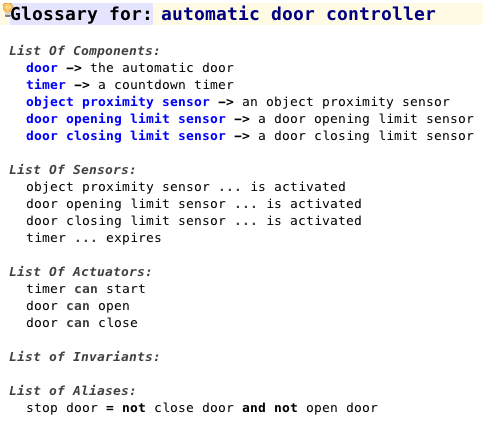
\includegraphics[width=.5\textwidth]{images/glossary.png}
     \caption{\textsf{EARS-CTRL} Glossary for sliding door
     controller}
     \label{fig:ears_glossary}
   \end{center}
 \end{figure} 
\vspace{-1cm}Note that in order to build requirements model illustrated in
figure~\ref{fig:ears_reqs} it is necessary to, as a first step, build a glossary
for the controller. An example of such a glossary is depicted in
figure~\ref{fig:ears_glossary}. The first section of an \textsf{EARS-CTRL}
glossary identifies the components of the system to be controlled. Each one of
those components contains actuators and (possibly) sensors that will be used by
the controller logic as (respectively) inputs from and outputs to the real
system. To allow for more ease of writing when building requirements, aliases
for logical expressions involving sensors or actuators can also be defined in
the glossary. More advanced users also have the possibility of defining
invariant relationships between sensors or actuators.
The vocabulary defined in the glossary is proposed to the requirements engineer
by the \textsf{EARS-CTRL} IDE in order to fill in the placeholders of an EARS
template when a new requirement being written.

Because well-formedness is enforced by construction, requirement specifications
written in \textsf{EARS-CTRL} are always syntactically correct.\vspace{-.4cm} 
\subsubsection{Simulation}
Once a controller has been synthesized from a set of EARS requirements, it
becomes important to understand whether it behaves as expected. In order to do
so we have used the Simulink engine~\cite{simulink} as a simulation back-end.
In figure~\ref{fig:ears_simulator} we display the \textsf{EARS-CTRL} panel that
allows ``playing'' the controller by providing a sequence of inputs manually.
Outputs are incrementally added to the panel as new inputs are provided by the
requirements engineer. Note that, because controllers have internal state,
the order in which the commands influences the controller's output. A ``Reset''
button in the panel allows resetting the controller to its initial
state.
\vspace{-.4cm}
\subsubsection{Generation of Test Cases}
\textsf{EARS-CTRL} allows generating test cases directly from the EARS
requirements. A test case consists of a sequence of $\langle
input, output \rangle$ pairs, where each input is a vector of sensor states
and each output a vector of actuator states. Note that individual sensors and
actuators can assume two states: \textsf{ON} or \textsf{OFF}. Test case
generation is configured by three parameters:\vspace{-.1cm}
\begin{itemize}
  \item \emph{Maximum test case length:} defines the maximum length of the
  $\langle input, output \rangle$ pair sequences to be generated.
  \item \emph{Allow parallel inputs:} enables or disables the possibility of
  having more than one sensor being active for inputs in the test case.
  \item \emph{Allow repeated inputs:} enables or disables having repeated inputs
  in the same test sequence. When enabled this parameter makes it such that
  an input vector cannot occur more than once in a test sequence -- thus
  limiting the length of test sequences to the number of possible input
  vectors.\vspace{-.7cm}
\end{itemize}
\begin{figure}[h!]
   \begin{center}
     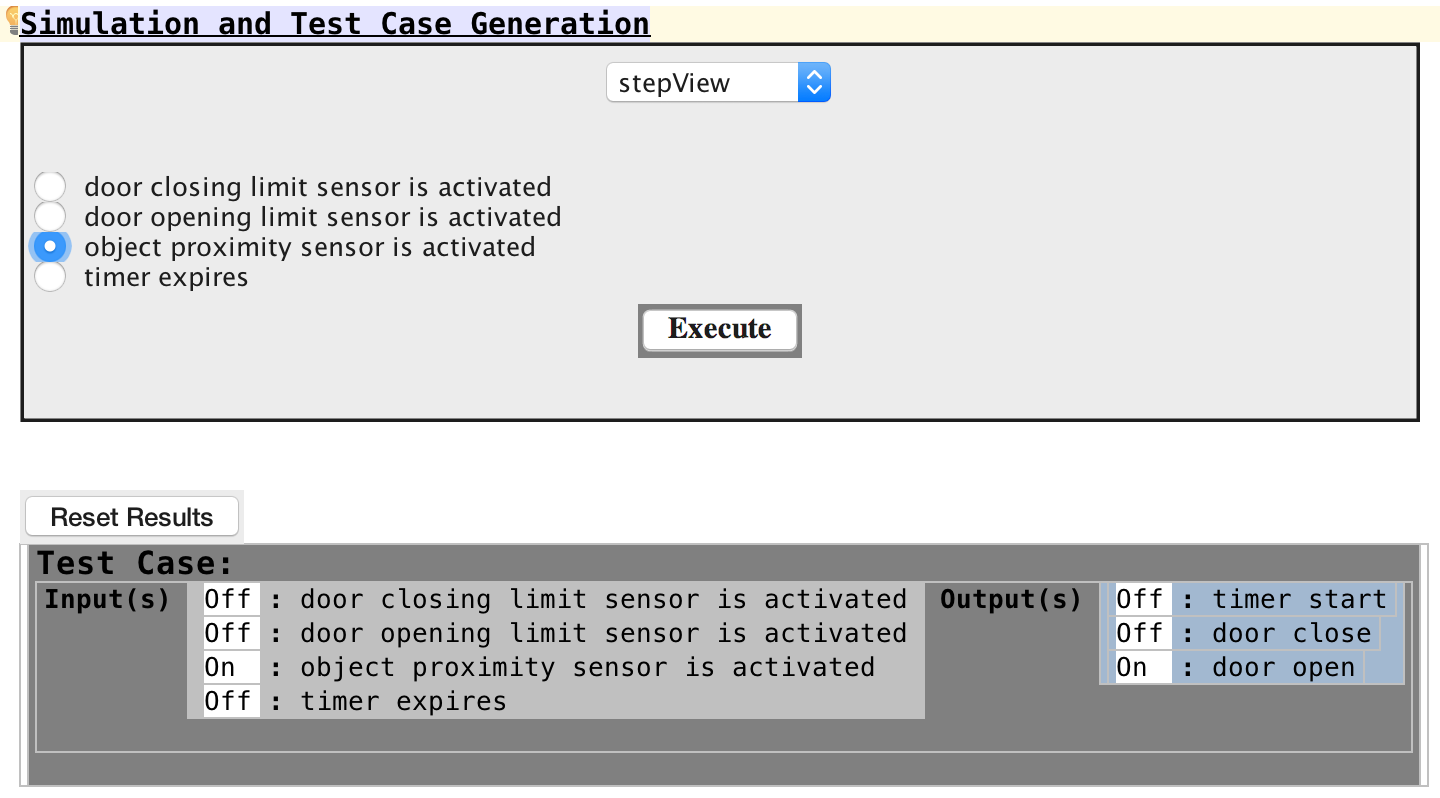
\includegraphics[width=.5\textwidth]{images/simulation.png}
     \caption{\textsf{EARS-CTRL} specification simulator\levi{sync picture
     with text}}
     \label{fig:ears_simulator}
   \end{center}
 \end{figure}
\vspace{-1cm}
Test cases generated by \textsf{EARS-CTRL} can serve two purposes: on
the one hand they are traces of execution of the synthesized controller and can
be used to make sure that controller behaves as expected; on the other hand one
may consider that the synthesizer is not trusted to generate controllers used in
production: in this case the synthesized controller can behave as an oracle to
generate test cases for a production controller implemented using alternative
means.\vspace{-.5cm}
\subsection{Code Generation}
\vspace{-.2cm}Although it is not possible to generate C code for the controller
directly from \textsf{EARS-CTRL}, this can be achieved by directly running Simulink's code
generator on the Simulink model obtained from an \textsf{EARS-CTRL} requirements
specification.
